In this chapter, we will introduce the general concepts and techniques behind Natural Language Processing. We will cover all the necessary steps for extracting meaningful topics from texts. Finally, a brief discussion about machine learning for tasks like classification and regression.


\section{Natural Language Processing}

	In artificial intelligence, NLP appears as the field responsible to study the interactions between computers and natural human language. Thus, it is capable of the program a computer to extract significant information from the text corpus, called documents, and use this information to apply a machine learning model and use it in several applications.

	\subsection{Text Processing Techniques}\label{sec:text-processing}

	The key task to several machine learning problems consists in make good data processing before applying any model. A clean data set can allow a model to increase its performance in the learning process, making a better identification of the patterns present in the variables. Therefore, in the following sections, it will be discussed a few techniques to clear the text and prepare it for machine learning algorithms.

	\subsubsection{Normalization}
	%https://www.kdnuggets.com/2017/12/general-approach-preprocessing-text-data.html

	There is no right way to normalize text. This process is crucially important to put all text at the same level. A normalization process consists of a series of steps to be followed consecutively, all of then can be seen as 4 big tasks: stemming, lemmatization, stop word removal, and everything else.

	\begin{enumerate}
		\item Stemming: is the process of reducing inflected words to a primitive form, the stem. This method can remove the word's affixes to capture its base meaning and still reducing the number of variations to save memory space. Figure \ref{fig:stemming} shows how some inflections for ``connect'' can be converted to its root form.

		\begin{figure}[h!]
			\centering
			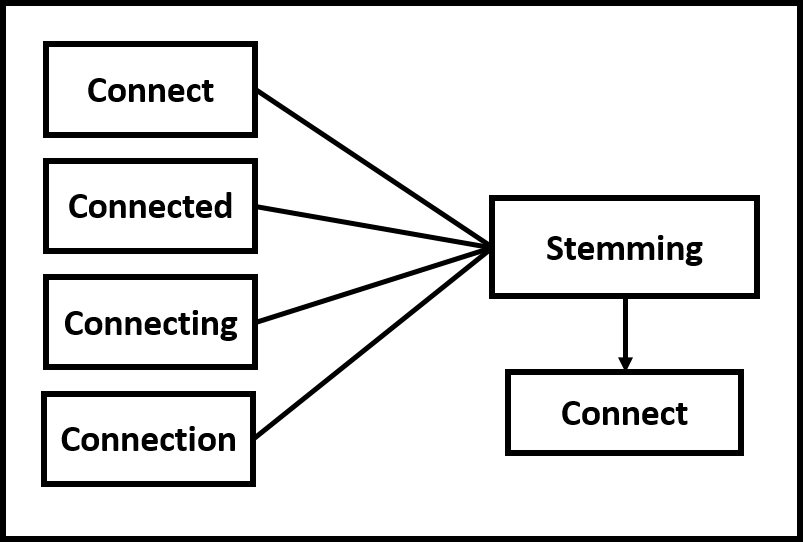
\includegraphics[width=0.45\linewidth]{01.Chapters/02.Background/stemming}
			\caption{Stemming process for ``connect'' variations. Figure adapted from \citeonline{vijayarani2015preprocessing}.}
			\label{fig:stemming}
		\end{figure}

		% stemming algorithms

		\item Lemmatization: similar to stemming, this step also reduces words to some primitive form, but with a little improvement. Lemmatization can return the words to its dictionary form, based on its part of speech context. Hence, it is possible to discriminate words with the same spelling but different meanings depending on the context.

		\item Remove stop words:
		many words can occur a several time in a document without adding any meaningful information, such as \textit{the}, \textit{is}, \textit{at}, \textit{which}, and \textit{on}. Their high frequency can be identified as an obstacle to perform good results on NLP models, \cite{kannan2014preprocessing}.

		The classic and easier method for eliminating stop words is based on using a pre-compiled list of well-known words and removing them from the text.
		But there still are some other techniques to remove stop words, most based on evaluating the frequency of words in the corpus, as described by \cite{vijayarani2015preprocessing}.

		A good way to perform it is by the Luhn's cut. From Zipf's law, the medium frequency words add more information, so we can cut off high and low frequency words, as shown in Figure \ref{fig:zipfs-law-and-luhns-proposed-cut-off-points}.

%		There are some types to remove stop words, most of then based on evaluating the frequency of words in a text, for more information see \cite{vijayarani2015preprocessing}.
%		But the classic and easier method is based on using a pre-compiled list of know words and removing then from the text.

		\begin{figure}[h!]
			\centering
			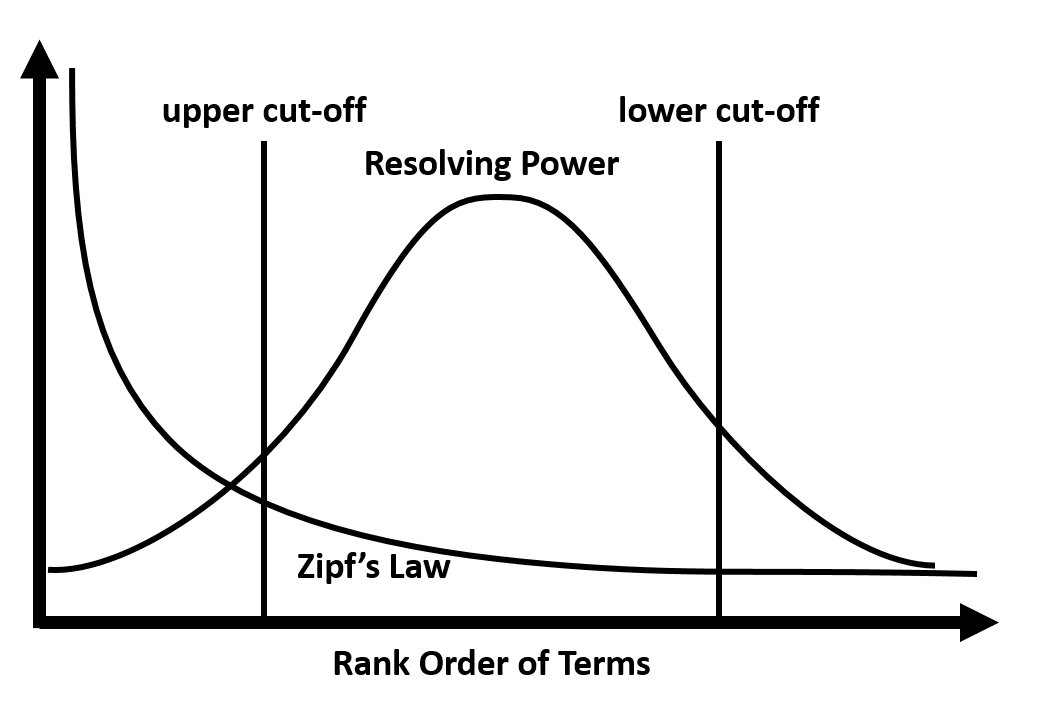
\includegraphics[width=0.5\linewidth]{01.Chapters/02.Background/Zipfs-law-and-Luhns-proposed-cut-off-points}
			\caption{Zipf’s law and Luhn’s proposed cut-off points. Figure adapted from \citeonline{cummins2006evolving}.}
			\label{fig:zipfs-law-and-luhns-proposed-cut-off-points}
		\end{figure}

		\item Everything else:
		different from the previous steps, the last one does not need any grammar rules or even a frequency analysis, it is purely text manipulation. It involves set all characters to lowercase; remove numbers or convert them to word form; remove punctuation; expand contractions; convert special characters to ASCII form; and any other conversion needed.
	\end{enumerate}

	\subsubsection{Tokenization}
	Once the data is normalized, we need to know how to represent it. The tokenization process consists of splitting longer strings into meaningful small pieces called tokens. The most common way to tokenize a text is chunking it into words, i.e., given a piece of text, the tokenization process will return a list of words.

	\subsubsection{Bag of Words}
	The machine learning algorithms take numerical features as input, hence, it will be necessary to represent the text in numerical form. With the Bag of Words model, we can represent in matrix form a set of documents.

	With the tokenization output, we will have the lists representations for all documents in the data set. Those lists can be interpreted as vectors over the vector space of all unique tokens, also called by vocabulary. So, for a given sentence, we mark how many times its words appear in the list indexes where each entry corresponds to a word in the vocabulary. Figure \ref{fig:bag-of-words} shows a simple example of how three sentences can be represented with the BoW model.

	\begin{figure}[h!]
		\centering
		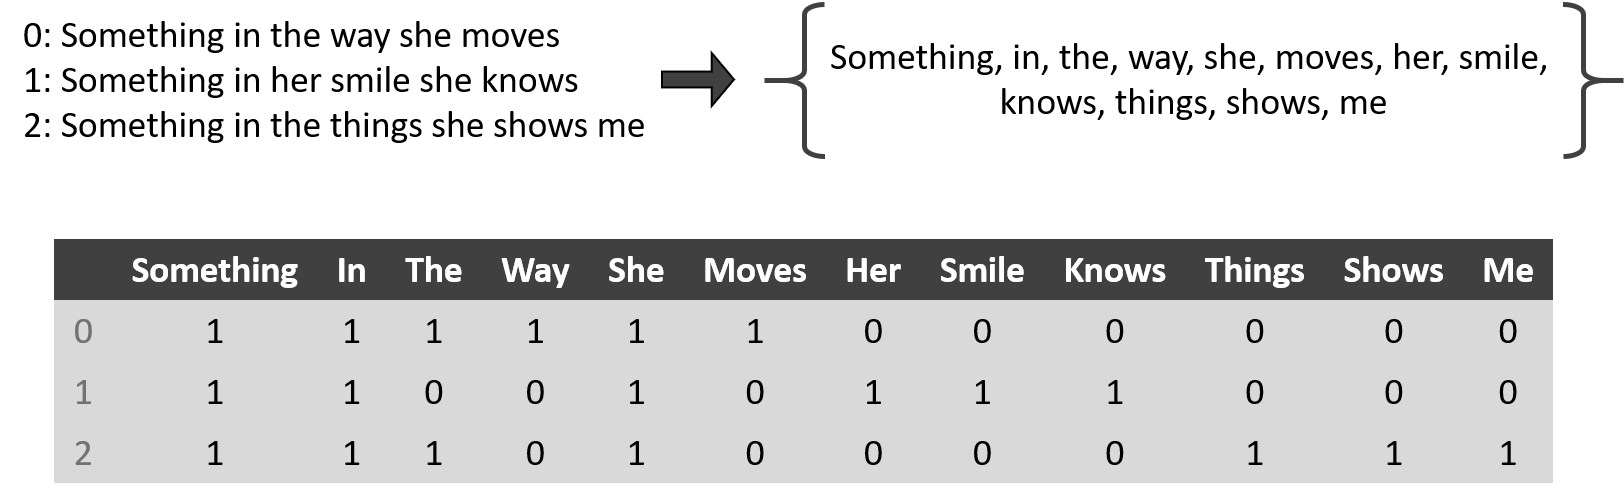
\includegraphics[width=\linewidth]{01.Chapters/02.Background/bag-of-words}
		\caption{Bag of Words example.}
		\label{fig:bag-of-words}
	\end{figure}

	\subsubsection{TF-IDF}

	Term Frequency Inverse Document Frequency, TF-IDF for short, is applied to a BoW to determine the relative frequency for words in a specific document when compared to the inverse proportion of that word over all documents in the collection. So, we can determine how important are the words in a specific document.

	From BoW, for the $i^{\text{th}}$ vocabulary's word in the $j^{\text{th}}$ document, its TF-IDF weight is
	\begin{equation}
	\label{eq:tf-idf}
	w_{i, j} = \text{tf}_{i, j} \times \log\left(\dfrac{N}{\text{df}_{i}}\right) \text{,}
	\end{equation}
	where the term frequency, $\text{tf}_{i, j}$, is how many times the $i^{\text{th}}$ word appears in the $j^{\text{th}}$ document. The document frequency, $\text{df}_{i}$, is the number of documents in which the $i_{\text{th}}$ vocabulary words is present. And, finally, $N$ is the size of the document collection, with a large number of documents this term can explode, so the logarithmic function is applied to dampen this effect.

	\subsection{Word Embedding}

	The vectorization methods like BoW and TF-IDF can be very useful, but they can not represent the context of the words. This means the same words used in different contexts have the same representation, just as different words used with the same meaning are represented differently. Besides that, an one-hot encoding method, like BoW, presents a very sparse representation with high dimensionality.

	Word Embedding is a technique to represent words in vectors capable of capture the words context in a document. It is also capable to smooth the high dimensionality effect by using a much more compact vector to represent the words.
	%We can use word embedding techniques as a text processing step before performing a classification, to archive better results.

	There are three most known ways to perform a good word embedding. We will describe briefly each one of them below.

	\subsubsection{Word Representations in Vector Space}

	The first great word embedding technique emerged when Google researchers proposed two architectures to build continuous vector representations of words. Word's context can be observed as the words that surround it in a sentence. Then, using shallow neural networks, it is possible to calculate the word vector space based on the word's context, \cite{mikolov2013efficient}.

	\begin{figure}[h!]
		\centering
		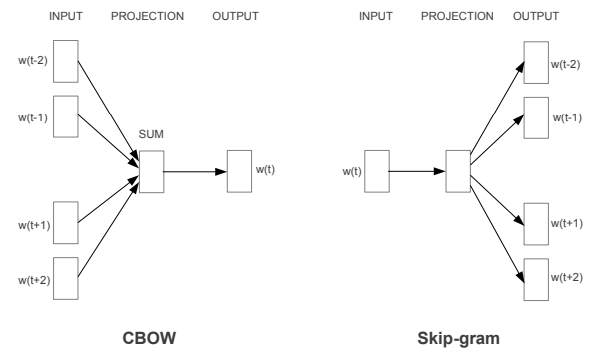
\includegraphics[width=0.8\linewidth]{01.Chapters/02.Background/word2vec_architectures}
		\caption{Word2Vec architectures. Figure adapted from  \citeonline{mikolov2013efficient}.}
		\label{fig:word2vecarchitectures}
	\end{figure}

	The first suggested approach is the continuous bag of words or CBOW, the left side of Figure \ref{fig:word2vecarchitectures} shows its architecture. Here the neural networks are designed to predict, given the context, which word is most likely to appear. So, words with the same probability to appear can assume a shared dimension in the words vector space.

	The second approach is known by Skip-Gram, architecture at right in Figure \ref{fig:word2vecarchitectures}. Very similar to CBOW, but instead of predicting the current word the Skip-Gram uses the current word as an input to a neural network to predict its context.

	After the network training process, we can use the hidden layer weight matrix as a lookup table to build the word embedding representation. The dimension for the vector space is managed by the number of neurons in the hidden layer.

	% INCREMENTO: Detalhes do artigo - base utilizada e testes

	\subsubsection{Global Vectors for Word Representation} %

	Just a year later \citeonline{pennington-etal-2014-glove} arrives with a new approach to represent words in a vector space. The Global Vectors for Word Representation, or GloVe, method emerged by the need to consider some factors ignored by Skip-Gram.

	Methods such as Skip-Gram learn their embedding by targeting words to their respective context, ignoring the fact that some words appear more in a context than others. Thus, this co-occurrence of words only adds more useless training examples, increasing the training complexity without adding relevant information.

	GloVe, however, proposes to use the corpus statistics more efficiently. Using a weighted least squares model trained on a global word-word co-occurrence counts matrix. Thereby, it is possible to build a lookup table for the words in vocabulary and use it to represent them in a vector space.

	% INCREMENTO: Explicar processo de montagem das co-ocorrencias e probabilidades

	\subsubsection{Word Vectors with Subword Information}

	Both Skip-Gram and GloVe provide a good vector representation for words, but there still is an unsolved problem, What to do with unknown words? To solve this question was proposed a new embedding technique which uses subword units to build a vector space, \cite{bojanowski2017enriching}.

	Similar to Skip-Gram, this new method, the FastText, train its embedding by using a target to predict the context. However, instead of using the full words, FastText goes a level deeper, breaking the words in $n$-grams, i.e., the word becomes its own context. The Figure \ref{fig:apple-tri-gram} shows how the word ``apple'' can be broken into $n$-grams.

	\begin{figure}[h!]
		\centering
		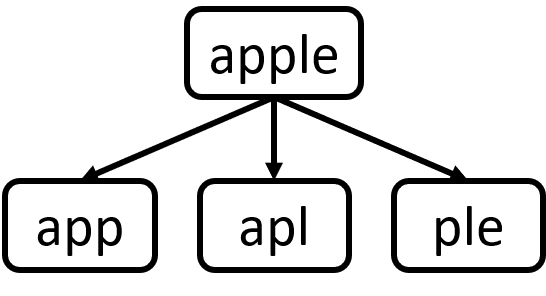
\includegraphics[width=0.4\linewidth]{01.Chapters/02.Background/apple-tri-gram}
		\caption{Tri-gram representation for ``apple'' word.}
		\label{fig:apple-tri-gram}
	\end{figure}

	There are a couple of great advantages to using this method. It is now possible to generalize new words or unseen in training data since they have the same characters as known ones. Although it is possible to use available pre-trained models, FastText requires less text to be trained, it can extract much more information from small pieces of text.

	\subsection{Topic Modeling}

	In text-mining, we often have document collections that we want to split into similar groups or even classify them related to each other. In this way, topic modeling is an unsupervised classification tool frequently used in text-mining to identify the hidden patterns, called ``topics'', in this document collection which carries consistent semantic meaning.

	Clustering methods, like hierarchical clustering, can be used to group the document collection into similar clusters. However, with a large amount of data a simple document clustering is not enough, because the semantic level of topics is not taken into account. To accomplish the topic modeling task a more sophisticated method is required, so methods like Latent Dirichlet allocation.

	Latent Dirichlet allocation, or LDA for short, is a probabilistic model that uses a Dirichlet distribution to model both the topics and the words. In LDA, each item in the collection is modeled as a mixture over an underlying set of topics. And the topics, in this way, are modeled as a mixture of words over the vocabulary, \cite{blei2003latent}.

	Without going too deep into the math behind the model, we can easily understand the two most basic principles that guide LDA. The first one said the documents are a mixture of topics which means that in a topic space each document could be interpreted as a linear combination of these topics, however, each one of the documents must be the most homogeneous as possible. The second principle said the topics are formed as a combination of words, i.e., documents about the same topics must share similar words, and also words distribution must be the most homogeneous as possible.

	Take the Figure \ref{fig:topicmodeling} as an example. It shows a little fictitious document set compounded for six words ``ball'' and ``match'' which can represent the Sports topic, ``pizza'' and ``pasta'' for the Food topic end, finally ``computer'' and ``phone'' for the Technology  topic. In this case, each word belongs to one topic, but that is not a rule, each topic is formed by a mix of words, and the documents a combination of topics.

	\begin{figure}[h!]
		\centering
		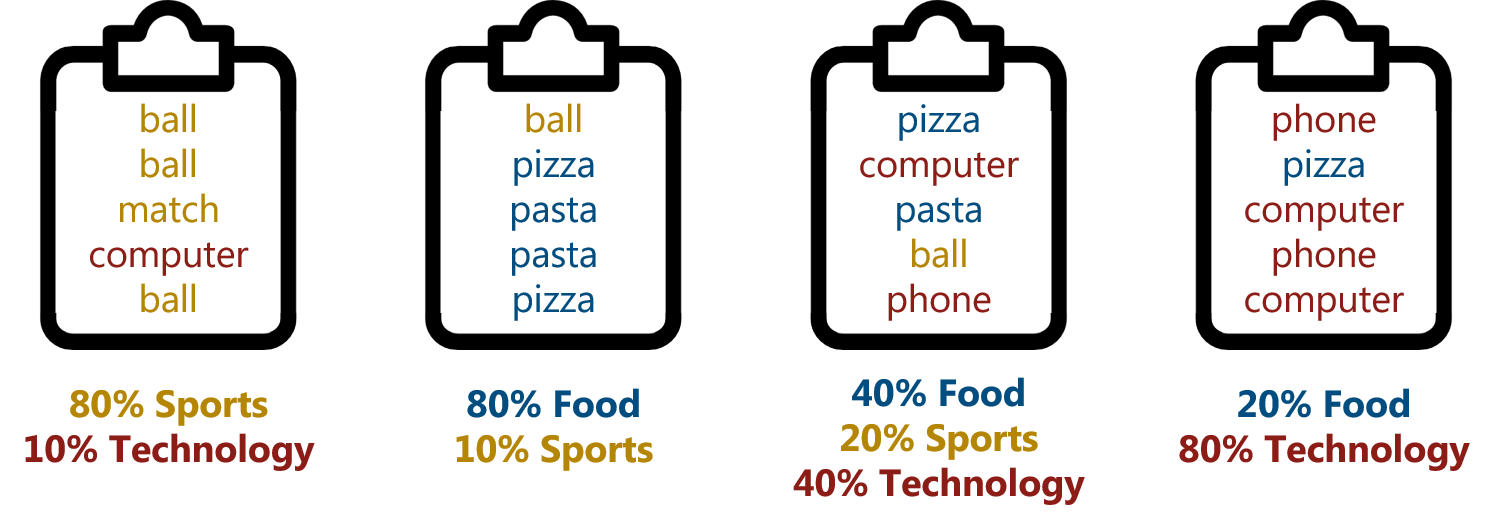
\includegraphics[width=\linewidth]{01.Chapters/02.Background/topic_modeling}
		\caption{Document collection modeled by topics.}
		\label{fig:topicmodeling}
	\end{figure}

	A final remark for the topic modeling algorithms is that the topic is not discovered by names, the machine only discovers the distribution of the words by topics but not which one is. It's human work to label the topic once they are found.

	\subsubsection{Generative Process}

	To better understand this model, we will analyze the generative process for creating the document collection illustrated by Figure \ref{fig:lda-generative-process}. Let's assume we have specified who the available topics are and their respective word distributions (far left), besides the topic proportions for each of the documents in the collection (the histogram at right).

	\begin{figure}[h!]
		\centering
		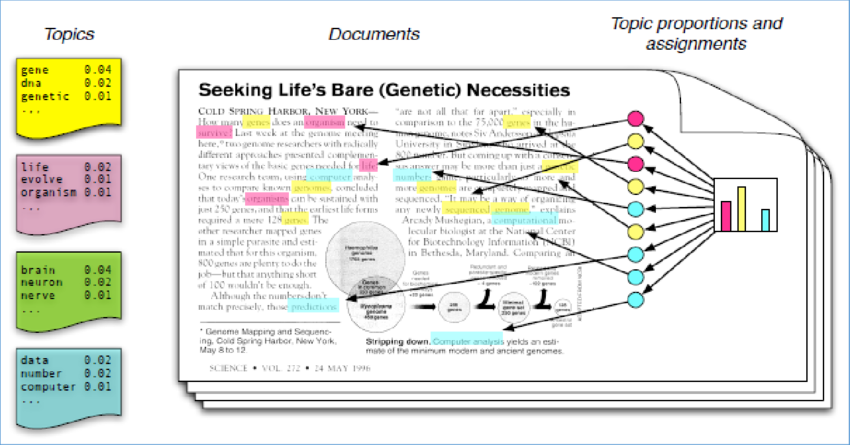
\includegraphics[width=\linewidth]{01.Chapters/02.Background/The-intuition-behind-LDA-Generative-process-by-D-Blei-17}
		\caption{The intuition behind LDA Generative process. Figure from  \citeonline{blei2012probabilistic}.}
		\label{fig:lda-generative-process}
	\end{figure}

	To generate a single document we choose its words as follows. Randomly choose a topic assignment from the topic distribution, then we choose the word from the corresponding topic. As shown by Figure \ref{fig:generative-probs} we can describe the generative process for the a given dirichlet parameters $\alpha$ and $\beta$.

	\begin{figure}[h!]
		\centering
%		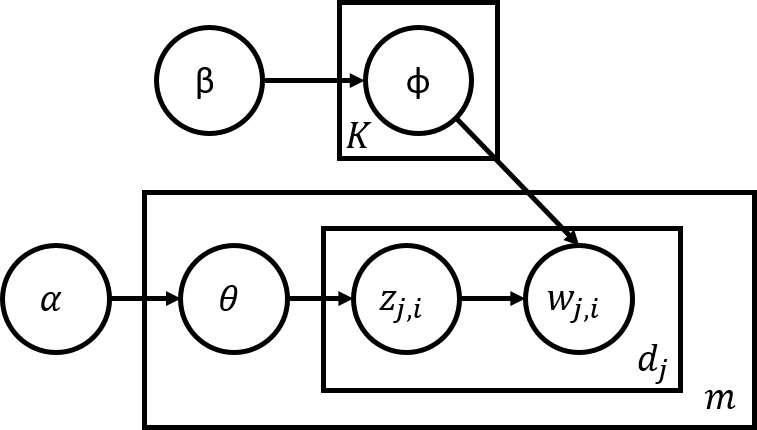
\includegraphics[width=0.5\linewidth]{01.Chapters/02.Background/generative-probs-stack}
		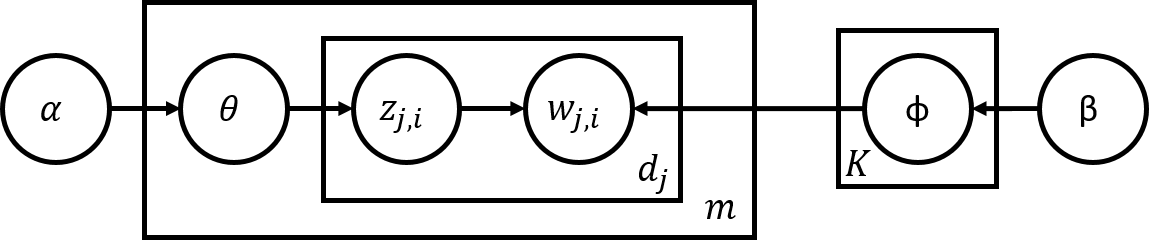
\includegraphics[width=0.7\linewidth]{01.Chapters/02.Background/generative-probs}
		\caption{Mathematical representation for LDA Generative process.}
		\label{fig:generative-probs}
	\end{figure}

	With that, we can model the generative process by
	\begin{equation}
		\label{eq:generative-lda}
		p(w|\alpha, \beta) = \prod_{k=1}^{K} p(\phi_{k}|\beta) \prod_{j=1}^{M} p(\theta_{j}|\alpha) \left( \prod_{i=1}^{V}p(z_{j,i}|\theta_{j}) p(w_{i,j}|z_{i,j},\phi_{z_{j,i}})  \right) \text{,}
	\end{equation}
	where $\phi$ is the distribution of $V$ words over the $K$ topics, $\theta$ is the topic distribution over the $M$ documents, $\alpha$ is the dirichlet parameter for $\theta$ distribution, and $\beta$ is the dirichlet parameter for $\phi$ distribution. The term inside the parentheses represent the choice of a word $w$ for a document given the assignment of topics $z$ for the specific document.
  % TODO: what is α and β?

	\subsubsection{Model Inference}

	The inference process for LDA consists of finding the best fit of the distribution $\phi$, for words over topics, the distribution $\theta$, for topics over documents, and the assignment $z$ for each document in the collection given the words vectors representation, in a bag of words format, and the hyperparameters $\alpha$ and $\beta$, who are the Dirichlet parameters for respective $\theta$ and $\phi$ distributions.

	Given the expensive computational cost, we can use some techniques to infer the LDA, the most common one is the Gibbs Sampling. This method is an algorithm for obtaining a sequence of observations which are approximated from a specified multivariate probability distribution. In easy words, showed by \citeonline{faleiros2016modelos}, the Gibbs sampler will iterate over the documents and its words to compute the relations
	\begin{equation}
		\label{eq:theta-dist}
		\theta_{k} = \frac{C_{w,k}^{\text{NWZ}} + \beta_{w}} {\sum_{w_{-i}} \left(C_{w_{-i},k}^{\text{NWZ}}
    + \beta_{w^{'}} \right)} \text{ and}
	\end{equation}
	\begin{equation}
		\label{eq:phi-dist}
		\phi_{d} = \frac{C_{d,k}^{\text{NZM}} + \alpha_{k}} {\sum_{k'}^{K} \left(C_{d,k^{'}}^{\text{NZM}} + \alpha_{k^{'}} \right)} \text{,}
	\end{equation}
	where $C_{w,k}^{\text{NWZ}}$ is the counter of times a word $w$ is assigned to topic $k$; and $C_{d,k}^{\text{NZM}}$ is the counter of times a topic $k$ is assigned to a word in a document $d$. Then, combining the relations from Equations \ref{eq:theta-dist} and \ref{eq:phi-dist} we have for the Gibbs sampler the relation:
	\begin{equation}
		\label{eq:gibbs-sampler}
		p(z_{i}=k|z_{-i}, \alpha, \beta, w_{i}) = \frac{C_{w,k}^{NWZ} + \beta_{w}} {\sum_{w_{-i}} \left(C_{w_{-i},k}^{NWZ} + \beta_{w^{'}} \right)} \cdot \frac{C_{d,k}^{NZM} + \alpha_{k}} {\sum_{k'}^{K} \left(C_{d,k^{'}}^{NZM} + \alpha_{k^{'}} \right)}\text{.}
	\end{equation}

	The Algorithm \ref{algo:gibbs-sampling} shows in a simple way how the Gibbs sampling works to infer the LDA distributions.

	\begin{algorithm}[h!]
		\caption{Gibbs sampler}
		\label{algo:gibbs-sampling}
		\begin{algorithmic}[1]
			\State \textbf{input:} number of topics $K$, document collection, $\alpha$ and $\beta$
			\Begin
			\State Initialize the counters $(\text{NWZ}, \text{NZM})$ randomly;
			\While{Did not converge}
			\For{document $m \in [1, D]$}
			\For{word $n \in [1, N_{m}]$ in document $m$}
			\State $\text{NWZ}[w_{m,n}, z_{m,n}]--$; $\text{NZM}[z_{m,n},m]--$;
			\State Sample a topic $z_{m,n}$ according to the Equation \ref{eq:gibbs-sampler}
			\State $\text{NWZ}[w_{m,n}, z_{m,n}]++$; $\text{NZM}[z_{m,n},m]++$;
			\EndFor
			\EndFor
			\If{converged since the last sampling}
			\State calculate the distributions $\theta_{k}$ and $\phi_{d}$ by Equations \ref{eq:theta-dist} and \ref{eq:phi-dist};
			\EndIf
			\EndWhile
			\End
		\end{algorithmic}
	\end{algorithm}

	\subsubsection{Evaluating Topic Models}

	After approximating LDA's distribution, we will have $K$ topics represented like distributions over the vocabulary. To interpret the found topics, we use the most likely words to co-occur, usually the top 10 or 15 with high probability. However, the $K$ parameter is a model input, so the wrong choice for it could result in unmeaningful topics.

	To evaluate properly the good interpretability for a topic model, there are some topic coherence metrics. The concept behind topic coherence consists of measuring the degree of semantic similarity between high scoring words in the topic. Then, a topic is considered to be coherent if its main words are related.

	There are several topic coherence metrics to evaluate interpretability for topic models, \citeonline{newman2010automatic} presents and compares some of them.
	% and \citeonline{rosner2013evaluating} studies	the $C_{\text{umass}}$ score based on document coocurrence counts.
	Despite this, according to \citeonline{syed2017full}, the coherence metric, labeled by $C_{\text{V}}$, achieves the highest correlation with all available human topic raking data. The calculation for $C_{\text{V}}$ metric is based on four steps:

	\begin{enumerate}
		\item Segmentation of the data into word pairs, combining each topic's top-N words with every other top-N word;

		\item Calculation of word or word pair probabilities, $p(w_{i})$ or $p(w_{i}, w_{j})$, respectively. That probability is calculated as the percentage of documents in which $(w_{i})$ or $(w_{i},w_{j})$ occurs, ignoring the frequencies and distances between words;

		\item Calculation of a confirmation measure $\phi$ that quantifies how strongly a word set supports another one, based on the normalized pointwise mutual information $\text{NPMI}$, for each segmented pair $S_{i}$. These confirmation measures can be calculated by:
		\begin{equation}
			\vec v (\text{W}') = \left\{ \sum_{w_{i} \in \text{W}'} \text{NPMI} (w_{i}, w_{j})^{\gamma} \right\}_{j=1,...,|\text{W}|} \text{,}
		\end{equation}
		\begin{equation}
			\text{NPMI} (w_{i}, w_{j})^{\gamma} = \left( \dfrac{\log \frac{P(w_{i}, w_{j}) + \epsilon}{P(w_{i}) \cdot P(w_{j})} }{- \log (P(w_{i}, w_{j}) + \epsilon) } \right)^{\gamma} \text{,}
		\end{equation}
		\begin{equation}
			\phi_{S_{i}}(\vec u , \vec w) = \dfrac{ \sum_{i=1}^{|\text{W}|} u_{i} \cdot w_{i} }{||\vec{u}||_{2} \cdot ||\vec{w}||_{2}} \text{,}
		\end{equation}
		where $\epsilon$ and $\gamma$ are parameters to, respectively, account the zero logarithm and place more weight on higher $\text{NPMI}$ values. The vector $\vec{v}(\text{W}')$ is called by context vectors.

		\item Finally, aggregation of individual confirmation measures into an overall coherence score, i.e., apply the arithmetic mean for all confirmation measures.
	\end{enumerate}

\section{Machine Learning}

	The basics behavior for a Machine Learning (ML) algorithm consists of building mathematical models based on data, usually known by training data, to provide predictions without being explicitly programmed to this, i.e., just knowing the training data, the model learns to make new predictions.

	When the entries for our training data have a label, used to guide the learning algorithm, we are facing a supervised learning method. Digging a little deeper, our problem could consist in classification when the labels are restricted to a limited set of values; or regression when the labels could have any numerical value in range.

	\subsection{Classification}

	As a usual ML problem, a classification task consists of building a model to fit some training data set. In a classification model, we make predictions for the class of given data points, when we have only two classes, let's call then by the positive and negative, we are facing a binary classification problem, \cite{pmlr-v81-menon18a}.

	There are several algorithms that we can use to build a classifier from the simple k-nearest neighbor until the more sophisticated ones like decision trees, naive bayes, support vectors machines, and artificial neural networks. Although each of these methods has its particularities in their formulation, they are capable of fitting the training data to make new predictions based on them.

%	\subsubsection{Naive Bayes}

%	\subsubsection{Support Vector Machine}

	\subsection{Evaluating a classifier}

	After the training step, we need to evaluate our classifier to verify how good our model is fitting the training data. The easiest way to evaluate our model is by reserving a split of the training set, the holdout set, exemplified in Figure \ref{fig:holdout-evaluate}. So, we use this unseen data to test the model and compute a metric.

	\begin{figure}[h!]
		\centering
		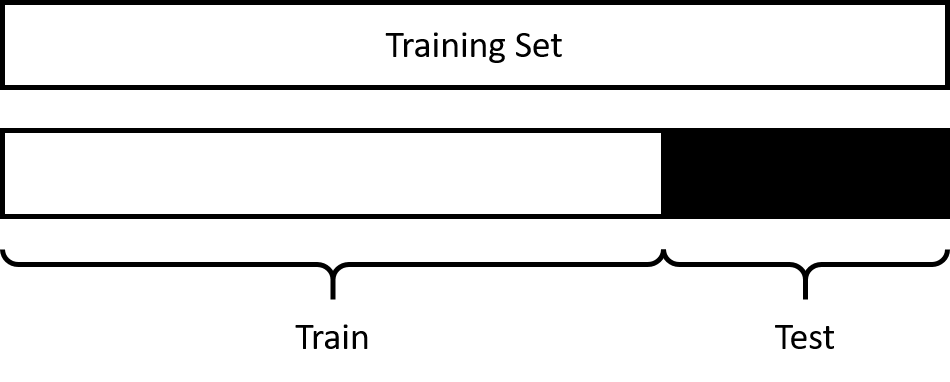
\includegraphics[width=0.5\linewidth]{01.Chapters/02.Background/holdout-evaluate}
		\caption{Train test split for holdout method.}
		\label{fig:holdout-evaluate}
	\end{figure}

	Another way to evaluate the model is through the $k$-fold cross-validation method, shown in Figure \ref{fig:cross-validate}. Dividing the data set into $k$ folds with the same size, we can train the model with $k-1$ folds and use the remaining one to test. Then we repeat this process to each fold and average the metric to evaluate the model, \cite{schaffer1993selecting}.

	\begin{figure}[h!]
		\centering
		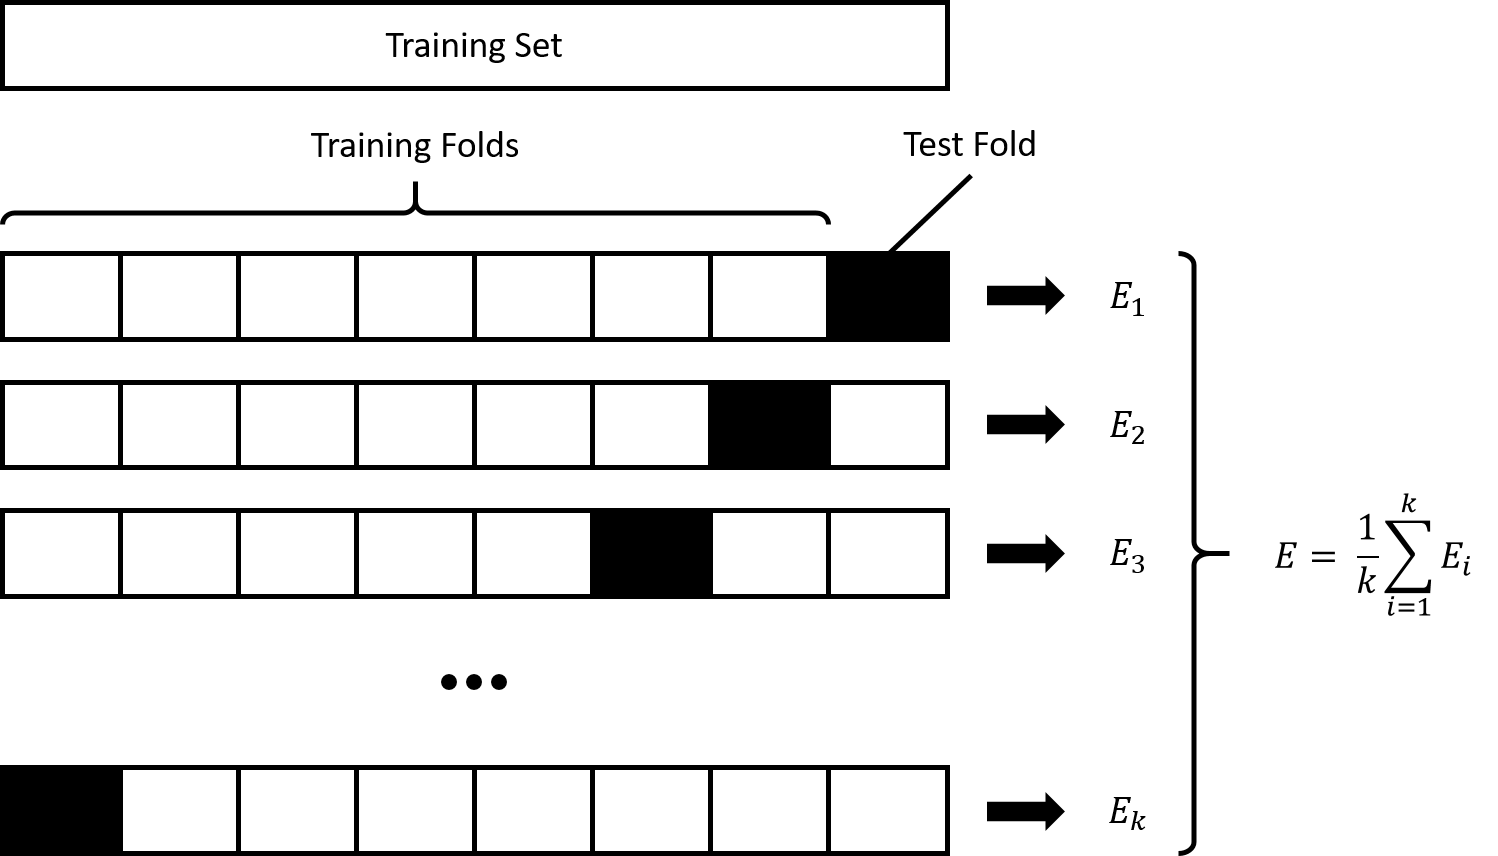
\includegraphics[width=0.6\linewidth]{01.Chapters/02.Background/cross-validate}
		\caption{Cross-validation process.}
		\label{fig:cross-validate}
	\end{figure}

	\subsubsection{Metrics}
	\label{sub-sub:metrics}

	Given the evaluation techniques, we still need a metric to properly evaluate the model, let us breifly review some metrics as shown by \citeonline{hossin2015review}. To present the main metrics, let's first take a brief look at the confusion matrix. Table \ref{tab:conf-matrix} exemplifies the confusion matrix for binary classification, each row represents the entries in a predicted class and the columns represent the actual class for the entry points.

	\begin{table}[h!]
		\centering
		\caption{Binary classification confusion matrix.}
		\label{tab:conf-matrix}
		\begin{tabular}{cc|c|c|}
			\cline{3-4}
			&          & \multicolumn{2}{c|}{Actual Class} \\ \cline{3-4}
			&          & Positive        & Negative        \\ \hline
			\multicolumn{1}{|c|}{Predicted} & Positive & TP              & FP              \\ \cline{2-4}
			\multicolumn{1}{|c|}{Class}     & Negative & FN              & TN              \\ \hline
		\end{tabular}
	\end{table}

	Thus, we can have the true positives (TP) and true negatives (TN) when our model makes a good prediction about the positive and negative classes, respectively, when the model misses the prediction we call false positive (FP) or false negative (FN).

	\begin{enumerate}
		\item \textbf{Accuracy:} The simplest metric, extracted from the confusion matrix, shows us the percentage of correct predictions by the relation:
		\begin{equation}
			\text{Accuracy} = \frac{\text{TP} + \text{TN}}{\text{TP} + \text{FP} + \text{TN} + \text{FN}} \text{.}
		\end{equation}

		\item \textbf{Precision:} In some cases, like a very imbalanced scenario, the accuracy is not good because even if the model predicts all the instances by the predominating class we will still have high accuracy. We define the precision of the positive class by:
		\begin{equation}
			\text{Precision}(P) = \frac{\text{TP}}{\text{TP} + \text{FP}} \text{.}
		\end{equation}

		Thus, we will analyze the true predictions only by the positive predicted class.

		\item \textbf{Recall:} This metric represents the fraction from a class that is correctly predicted. We define the recall for the positive class by:
		\begin{equation}
			\text{Recall}(P) = \frac{\text{TP}}{\text{TP} + \text{FN}} \text{.}
		\end{equation}

		Similar to precision the recall for the positive class will compare the true predictions by the total count of true actual classes.

		\item \textbf{F1 Score:} In some cases, we may want to give the same importance to both precision and recall. A popular metric to combine then is called F1-score, which is the harmonic mean of precision and recall. We define the F1-score for the positive class by:
		\begin{equation}
			F1(P) = \frac{2 \times \text{Precision}(P) \times \text{Recall}(P)}{\text{Precision}(P) + \text{Recall}(P)} \text{.}
		\end{equation}

	\end{enumerate}


